%  !TeX  root  =  user_guide.tex

\section{Plugin decorativi}

% when the revision of a section has been finalized,
% comment out the following line:
% \updatedisclaimer

I plugin decorativi includono il plugin Etichetta Copyright, il plugin Freccia nord ed il plugin 
Barra di scala. Sono usati per "decorare" la mappa aggiungendo elementi cartografici.

\subsection{Plugin Etichetta Copyright}\label{copyrightlabel}

Il nome del plugin è un po' fuorviante, in realtà si può aggiungere qualsiasi testo alla mappa.

\begin{figure}[ht]
   \centering
   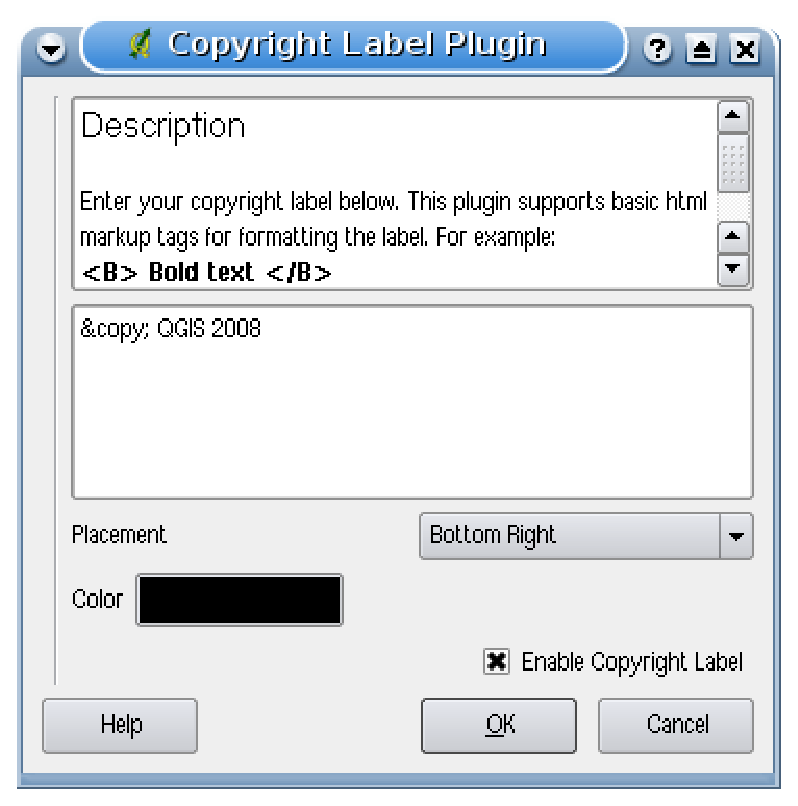
\includegraphics[clip=true, width=7cm]{copyright}
   \caption{Plugin Etichetta Copyright \wincaption}\label{fig:copyright}
\end{figure}

\begin{enumerate}
\item Assicurarsi che il plugin sia caricato
\item Cliccare su \mainmenuopt{Plugins} \arrow \dropmenuopt{Decorazioni} \arrow \dropmenuopttwo{copyright_label}{Etichetta Copyright} 
o sul pulsante \toolbtntwo{copyright_label}{Etichetta Copyright} nella barra dei plugin.
\item Digitare il testo che si vuole aggiungere alla mappa. Si può usare codice HTML come mostrato nell'esempio
\item Scegliere il posizionamento dell'etichetta dal menu a tendina \selectstring{Posizione}{In basso a destra}
\item Assicurasi che la casella di controllo \checkbox{Abilita etichetta di Copyright} sia selezionata
\item Cliccare \button{OK} 
\end{enumerate}

Nell'esempio, la prima linea è in grassetto, la seconda (creata usando \textless br\textgreater) 
contiene un simbolo di copyright, seguito dal nome della nostra compagnia in corsivo.

\subsection{Plugin Freccia nord}\label{northarrow}

Il plugin Freccia nord aggiunge alla mappa una semplice freccia indicante il nord. Al momento 
c'è un solo stile disponibile. Si può modificare manualmente l'angolo della freccia o lasciare 
che QGIS imposti automaticamente la direzione. 
Per il posizionamento della freccia si hanno quattro possibilità, corrispondenti ai quattro angoli della mappa.

\begin{figure}[ht]
   \centering
   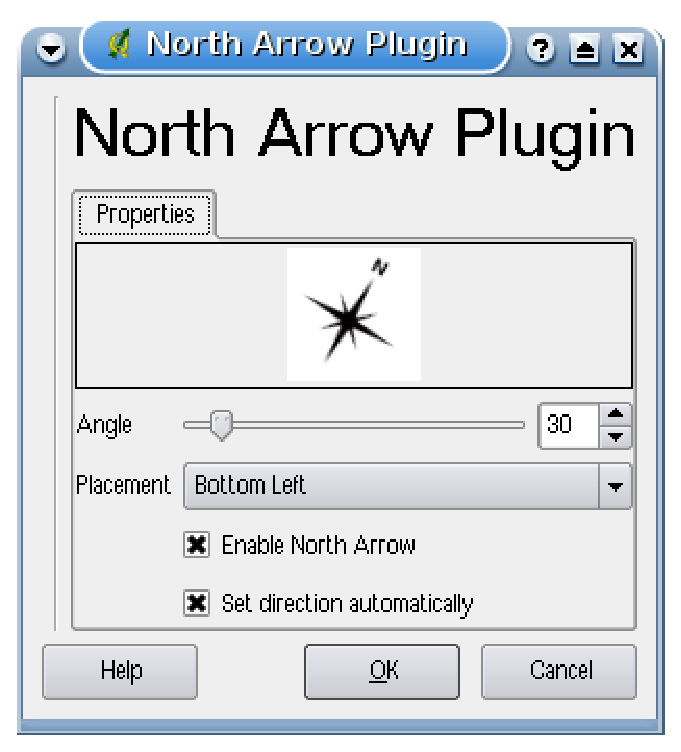
\includegraphics[clip=true, width=8cm]{north_arrow_dialog}
   \caption{Plugin Freccia Nord \wincaption}\label{fig:north_arrow}
\end{figure}

\subsection{Plugin Barra di Scala}\label{scalebar}

Il plugin Barra di scala aggiunge una semplice barra di scala alla mappa. Si può controllare 
lo stile ed il posizionamento, come anche l'etichettatura della scala.

QGIS supporta solamente la visualizzazione della scala nella stessa unità di misura della mappa. 
Se l'unità di misura dei layer è il metro, non si può creare una barra di scala in piedi.
Allo stesso modo, se si usano gradi decimali, non si può creare una barra di scala che 
mostri le distanze in metri.

Per aggiungere una barra di scala:

\begin{enumerate}
\item Cliccare su \mainmenuopt{Plugins} \arrow \dropmenuopt{Decorazioni} \arrow \dropmenuopttwo{scale_bar}{Barra di Scala} 
o sul pulsante \toolbtntwo{scale_bar}{Barra di Scala} nella barra dei plugin.
\item Scegliere il posizionamento dal menu a tendina \selectstring{Posizionamento}{In basso a sinistra}
\item Scegliere lo stile dalla lista \selectstring{Stile della Barra di Scala}{Porta in basso}
\item Scegliere il colore della barra di scala \selectcolor{Colore della barra}{black} o usare il colore nero di default
\item Impostare la dimensione della barra e la sua etichetta \selectnumber{Dimensione della barra}{30 gradi}
\item Assicurarsi che la casella di controllo \checkbox{Abilita barra di scala} sia selezionata
\item Se si vuole, scegliere di arrotondare automaticamente il numero quando la mappa viene ridimensionata 
\checkbox{Arrotonda automaticamente il numero durante il ridimensionamento}
\item Cliccare \button{OK} 
\end{enumerate} 

\begin{figure}[ht]
   \centering
   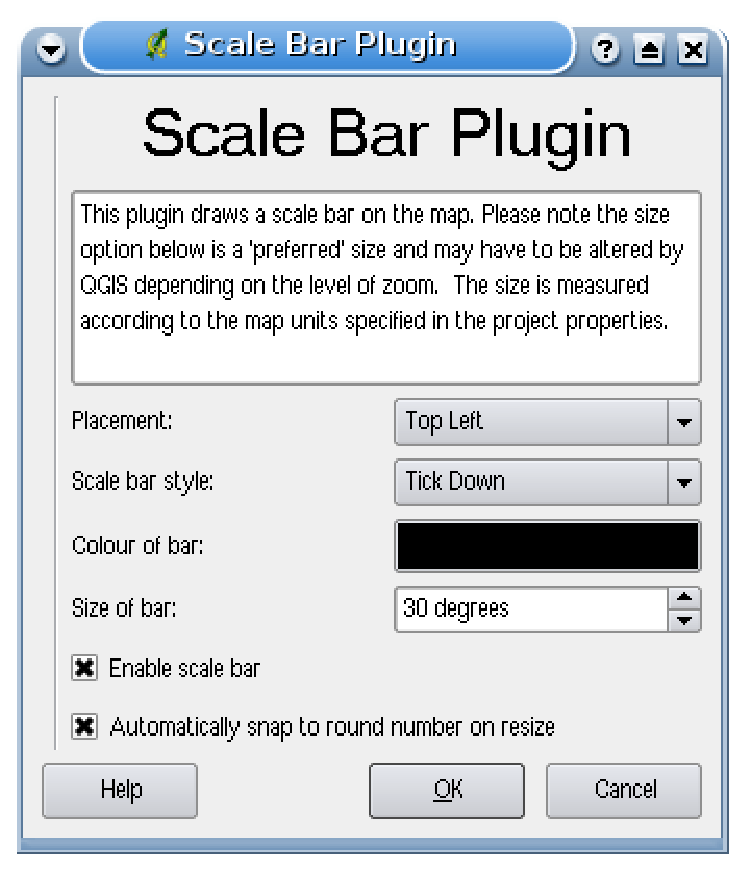
\includegraphics[clip=true, width=8cm]{scale_bar_dialog}
   \caption{Plugin Barra di scala \wincaption}\label{fig:scale_bar}
\end{figure}

\begin{Tip}\caption{\textsc{Impostazioni dei plugin salvate nel progetto}}\index{plugins impostazioni}
Quando si salva un progetto .qgs, ogni impostazione dei plugin decorativi viene salvata nello stesso 
progetto e ripristinata alla successiva apertura del file .qgs.
\end{Tip}

\FloatBarrier
